\chapter{Literature Review}

In an time of austerity and double dips in the economy, \gls{IB} is playing `the game' not only over products and customers but also with institutions. Companies like Apple and Samsung are  fighting in court over~\gls{IP} in a multitude of countries. The cell phone department of Motorola was bought by Google solely because of it's numerous \glspl{IP}. The field not limited to \glspl{IP}. Next to the fight over \gls{IP} subsidies are at the forefront of the public debate as well. Boeing and Airbus have been fighting over subsidies for decades where on more than one occasion the \gls{WTO} has ruled on the validity of these subsidies. More recently solar panels have become a topic of tariffs between the European Union and China. \\

The field of play is governed by governments, trade blocks and the \gls{WTO} on the one hand and \gls{IB} on the other.
A multitude of forces are acting on this playing field and the different actors on this pitch have to cooperate. 
Different \gls{MNE} will cope differently with the challenges that are set by the institutions and the environment that they are operating in. That this environment is of importance is explained by \gls{IBV}~\cite{Kostova:1999,Meyer:2009,Wang:2012} 

\section{History of Strategy in IB Literature}
Using the examples of Google, Apple, Samsung, Boeing and Airbus strategies of the large~\mne have extended. It is no longer just resources and industries that dictate the strategies that companies employ. 
According to~\cite{Peng:2009}, the market-based institutional framework has been taken for granted, and formal institutions (such as laws and regulations) and informal institutions (such as cultures and norms) have been assumed away as``background''.

This trent has given rise to what~\cite{Peng:2009} calls the `third leg' of the strategy tripod.~\Gls{IBV} has been an addition to the theories of~\gls{RBV} introduced by~\cite{Barney:1991} and industry based view by~\cite{Porter:1980}. 
Since being introduced by~\cite{Porter:1980} (Industry based view) and~\cite{Barney:1991} (~\gls{RBV}) strategic management (theory) or strategy in short, has gained a lot of momentum in the international business community. \\ 

\subsection{\glsdesc{InBV}}
The industry based view is known for the five forces (see figure~\ref{fig:5forces}), which states that choosing the correct industry is the key to gaining competitive advantage. The competitiveness of a firm is determined by the five \emph{external} forces.

\begin{figure}[htbp]%
       \centering%
	\includegraphics[width=0.7\textwidth]{5forces}%
 	\caption{Five Forces from~\cite{Porter:1980}}%
 	\label{fig:5forces}%
\end{figure}

\subsection{\glsdesc{RBV}}

\Gls{RBV} came as a response to~\cite{Porter:1980} a decade later.~\Gls{RBV} argued that a firms strategic advantage is depended on it's heterogeneous resources (a bundle of all assets, knowledge, and capabilities) which have to be
\begin{enumerate}[(a)]
\item must be valuable, in the sense that it exploit opportunities and/or neutralises threats in a firm’s environment
\item must be rare among a firm’s current and potential competition, 
\item must be imperfectly imitable
\item  there cannot be strategically equivalent substitutes for this resource that are valuable but neither rare or imperfectly imitable 
\end{enumerate} 
In contrast to~\gls{InBV} the theory of~\cite{Barney:1991} is~\emph{extrospective}. 
The theory by~\cite{Barney:1991}  has been given the acronym VRIN\@.\\

However~\gls{RBV}, which in introspective in nature and \gls{InBV} is extrospective can not account for the entire spectrum. These are the formal and informal rules of the game~\cite{North:1990}. In the 2010s in the Netherlands a new breed in chicks (a broiler) was bread. From a scientific standpoint this was a very successful product with regard to sustainability and food conversion. 
This `plofkip' (in English BangChick) as it was rebranded by the media and animal welfare organisations has certain traits that are very positive\footnote{taken from websites (\url{http://fransvdst.wordpress.com/2012/10/28/het-duurzame-vleeskuiken})}\footnote{Dutch newspaper `Trouw'
(\url{http://www.trouw.nl/tr/nl/5948/Dierenwelzijn/article/detail/3267278/2012/06/07/De-voordelen-van-de-plofkip.dhtml}) 
and (\url{http://www.trouw.nl/tr/nl/4332/Groen/article/detail/3324936/2012/10/01/Vanuit-het-milieu-gezien-is-er-niets-mis-met-plofkip-en-megastal.dhtml})}
\newpage
These chicks had the following advantages:


\begin{itemize}
\item The broiler grows faster than the free-range chicken carcass weight (40 days vs. 56 days) and need to be fed so less time and therefore needs to be less manure removed
 \item    The broiler grows better with less feed than the free-range chicken (has better feed conversion called). There is the free-range chicken so need more feed to grow. One kilogram of meat
\item     The broiler has less stable space at his disposal including what should be heated
\item     The manure of a broiler remains in the stable and is thus more environmentally friendly processes
  \item   The broiler is so tender and cook faster
\end{itemize}
Despite all these advantages, the disadvantages (cleverly supported by pictures) that the chickens had such difficulties as supporting their own bodyweight and their harts having issues coping with the high growth rate~\footnote{taken form \url{http://www.wakkerdier.nl/actueel/plofkip-campagne and translated freely by the author}}, the broiler had to be abandoned and is no longer `in play' as a food source.\\
The aforementioned example can not be explained by the theories by~\cite{Porter:1980,Barney:1991} do not cover this phenomenon. The lack of context and the power of institutions are not catered for.  

\subsection{\glsdesc{IBV}}
 
 Context and institutions are the prevalent terms when it comes to \ibv. 
 %%% INSTITUTIONAL BASED VIEW EZplaing
The institutional based view dictates that firms performance and choices do not only depend on resources and the industry the firm is competing in, but also depends on the environment in which it is operating. 
This environment is the context that has been mentioned before.
Context is the third leg~\cite{Peng:2009} that influences the various decisions that firms have decide on in~\ib. 
These institutions present themselves in two forms `formal' and `informal'. 
So~\ibv~takes into account not only strategic choices driven by industry conditions and firm-specific resources, that traditional strategy research emphasises (~\cite{Porter:1980,Barney:1991}), but are also a reflection of the formal and informal constraints of a particular institutional framework that decision makers confront (\cite{Oliver:1997,Scott:1995}). 

~\ibv~is supported by two forces; external and internal in nature according to~\cite{Peng:2009}. 
The latter is the institutionalism movement by the likes of economist~\cite{North:1990} and sociologist like~\cite{DiMaggio:1983,Scott:1995}. 
These institutions are known as the rules of the game.
More on the theory of institutions will be investigated in section #ref.\\

The internal forces that underpin~\gls{IBV} are a reaction to criticisms on the theory of~\gls{InBV} of a lack of awareness of context~\cite{Narayanan:2005}. 
Under certain circumstances for example, the pursuit of cost leadership can be deemed unethical in that the raising broilers however sustainable were seen as cruel by modern animal welfare standards. 
Some times the cost-leadership strategy can drive companies to engage in (illegal) price fixing actions. 
In the Dutch mobile phone market, the telecom providers (KPN, Vodafone and T-mobile) have been reprimanded twice in the last decade or so by the \gls{ACM}\fn{The \gls{ACM} is the new name for the \gls{NMA} witch is the Dutch regulatory agency for competitions, comparable tot the British \gls{OFT} (soon to be \gls{CMA}) } for price fixes deals on mobile calling costs\fn{Sourced from \url{http://www.volkskrant.nl/vk/nl/2844/Archief/archief/article/detail/3067315/2011/12/07/Mobiel-bellen-blijkt-te-duur-door-kartel.dhtml}}. \\

\cite{Kraaijenbrink:2009} also summarised \gls{RBV} critiques in his 2009 paper. 
He concluded that it is mainly the definition of `resource' and `valuable' in combination with the lack of acknowledgement of the combination of bundling resources and the human involvement, that is undermining strength of \gls{RBV}.
Likewise~\cite{Priem:2001} concluded that the contexts are missing from \gls{RBV}, where~\cite{Dung:2012} states that the ``resource-based view often neglects the issues of strategy implementation, i.e., various activities through which competitive advantage is directly created. Some resources may be valuable and rare at some point in time, this can change in an instant." 
Take a look at the operating system that Nokia used in its mobile phones in the early 2000s. 
This was considered the peak of user-friendliness; until the iPhone came along. 
The rare resource of a user-friendly operating system and user interface became defacto obsolete hence non-valuable.\\

The \ibv~tries to come up with an answer to these critiques. 
Externally, the rise of new institutionalism throughout the social sciences has energised scholarly attention in strategy to focus on how institutions matter. Internally, the frustration associated with the industry-based and resource-based views’ lack of adequate attention to contexts has called for new theoretical perspectives that can overcome these drawbacks. 
The result is the emergence of the institution-based view~\cite{Peng:2009} (see picture~\ref{fig:ibv}).


\begin{figure}[htbp!] 
      \label{fig:ibv2}
	\centering
	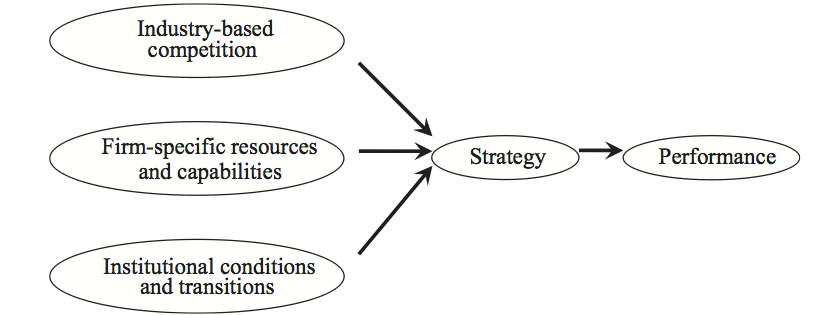
\includegraphics[width=0.65\textwidth]{Peng2009.pdf}
 	\caption{The Institution-Based View as a Third Leg for a Strategy Tripod. Source:~\cite{Peng:2009}}
\end{figure}

The figure shows the dependance on both the theories of~\cite{Barney:2001} and~\cite{Porter:1980} for~\ibv. Obviously~\ibv is not an attempt to dismiss other theories more an attempt to complete theories on strategy as they exist at the moment. Strategy is about making the right choices at the correct moment. \\
Given the influence of institutional frameworks on firm behaviour, any strategic choice that firms make is inherently affected by the formal and informal constraints of a given institutional framework (North, 1990; Oliver, 1997). 
Strategy literature does not take into account the institutional frameworks that influence the choices \mne have to take. 
Strategic literature does not discuss the specific relationship between strategic choices and institutional frameworks~\cite{Peng:2008}.
Treating institutions as independent variables, an institution-based view on business strategy, therefore, focuses on the dynamic interaction between institutions and organisations, and considers strategic choices as the outcome of such an interaction (see figure~\ref{fig:ibv})\cite{Peng:2002}.
Not only have more scholars come to realise that institutions matter~\cite{Powell:1991,Scott:1995}, but also that strategy research cannot just focus on industry conditions and firm resources.~\cite{Khanna:1997}\\


%


\begin{figure}[htbp!]
	\centering
	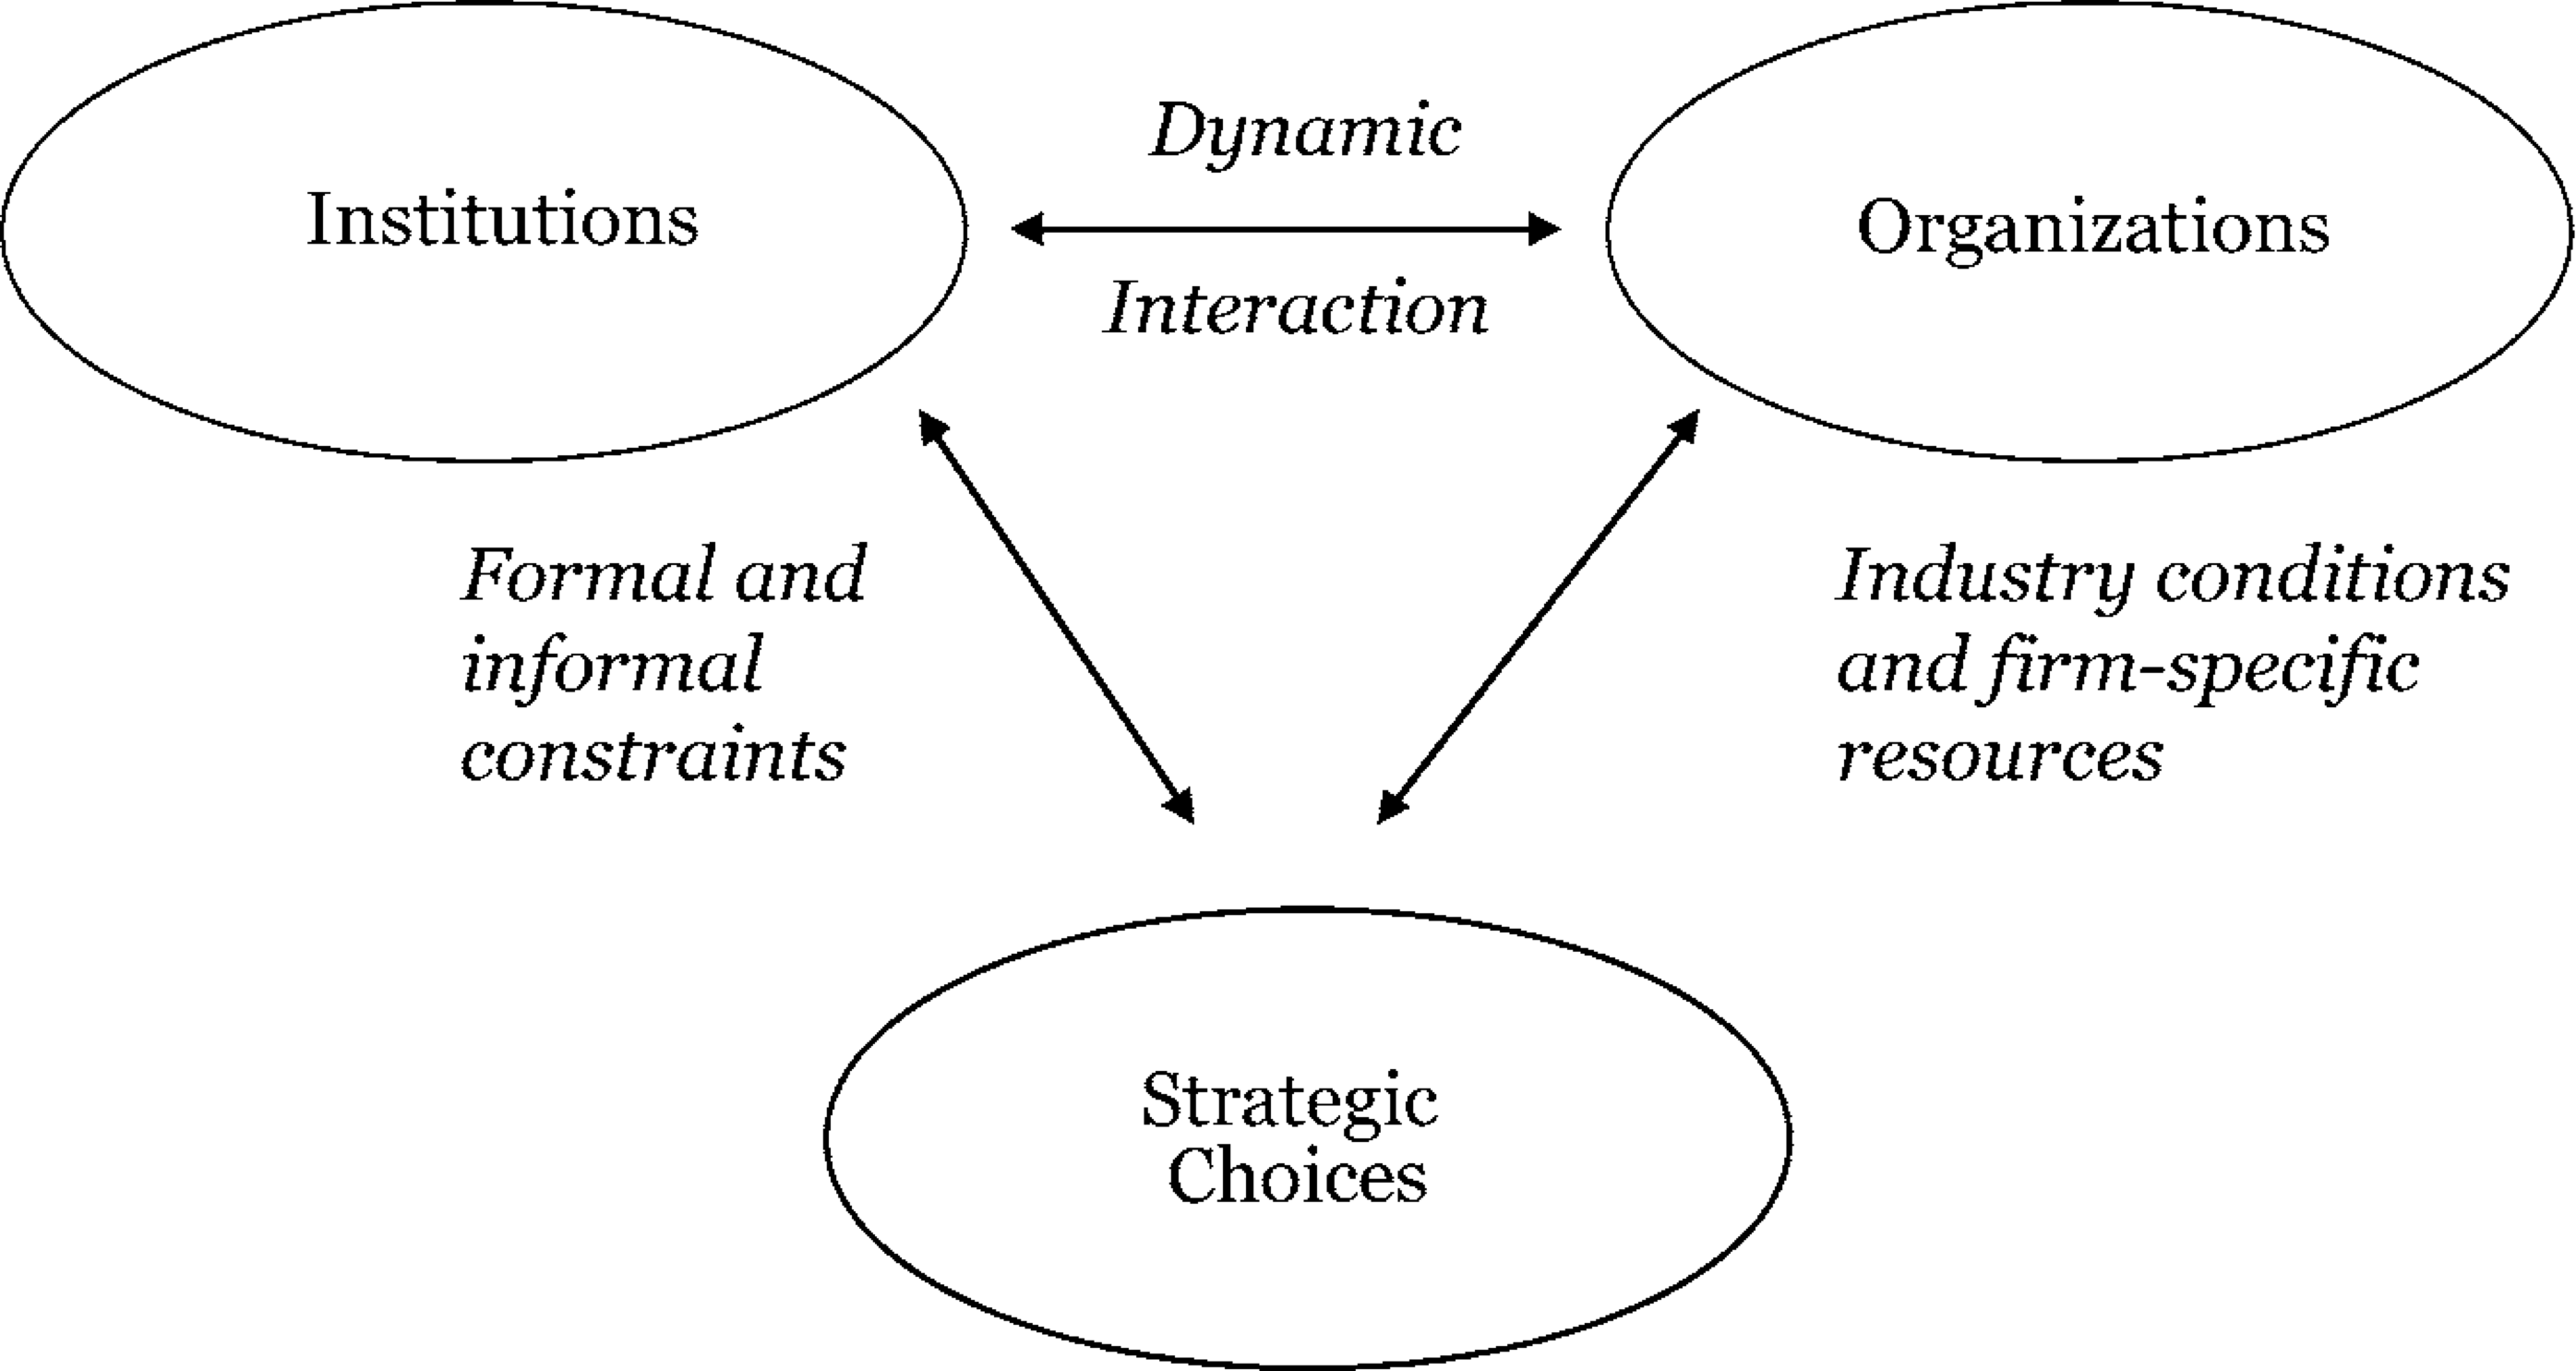
\includegraphics[width=0.65\textwidth]{IBV.pdf}
 	\caption{Institutions, organisations, and strategic choices. Source:~\cite{Peng:2000}}
 	\label{fig:ibv}
\end{figure}



When markets work smoothly in developed economies, ``the market-supporting institutions are almost invisible". mcMillan2007


The effect of institutions on strategy can be seen most obviously in the asian economies~\cite{Peng:2002}.











These institutions are influencing the decision making process in~\gls{IB}.  The dynamic that takes place is depicted in picture~\ref{fig:ibv}. 


So~\ibv~is cannot consist by itself but needs \rbv~\cite{Barney:1991} and~\cite{Porter:1980} as is shown in figure~\ref{fig:ibv}. 
Where \rbv looked solely at the firm in a set environment \ibv also takes the surroundings into account. These surroundings are the institutions that govern the environment the \mne is playing the game. 
The actions of institutions can be divided into three pillars. Compliance from the firms occurs through \\(1) expedience (regulative pillar or coercive \iso),\\
 (2) social obligation (normative pillar or normative \iso), or \\
 (3) on a taken for granted basis (cognitive pillar) or mimetic \iso~where organisations respond to uncertainty by adopting patterns of other organisations that are deemed `successful'~\cite{Westney:2005,Peng:2008,Kostova:1999,DiMaggio:1983,Scott:1995}.\\ 
\mne conform to these pillars or isomorphisms because these provide legitimacy~\cite{Powell:1991}

Although firms take decisions on the individual resources and capabilities~\cite{Barney:1991} the influence of institutions can no longer be ignored. This is the difference between~\rbv and~\ibv. 







\section{Institutional Theory}


Following~\cite{North:1990}, we understand institutions as ``humanly devised constraints
that structure human interaction". Institutional factors function as the formal and
informal ``rules of the game'' that socially constrain contracting practices between the \gls{BoD} and 
executives (\cite{North:1990}).
These formal en informal constraints operate in structures for both social and economic exchanges. 
Institutions are pervasive in that they are capable of shaping the behaviours of multiple actors (i.e. 
individuals, firms, industries, and~\glspl{NGO}). More broadly speaking, institutions serve to reduce 
uncertainty for different actors by conditioning the ruling norms of firm behaviours and defining the 
boundaries of what is considered legitimate.~\cite{Peng:2008}\\



According to~\cite{Peng:2003} unfortunately, little is known about how organisations make strategic choices when confronting such large-scale institutional transitions.


 Firms do not only have to look at their resources and capabilities~\cite{Barney:1991}, but have to look at ``the rules of the game''~\cite{Scott:1995}. These so called rules include the environment that the firm \mne~has to adhere to.\\




The central argument is that “organisations conform to the rules and beliefs systems in the environment because this isomorphism (regulatory, cognitive and normative) earns them legitimacy.

Not only have more scholars have come to realise that institutions matter and, that strategy research cannot just focus on industry conditions and firm resources alone~\cite{Powell:1991,Scott:1995}.

Nowadays institutional theory appears to be a highly insightful approach when probing into organisational strategies in Asia~\cite{Hoskisson:2000}.

\Gls{IB} has long been a favourite topic in academic literature. The term \gls{IB} alone gives over 2M hits in Google Scholar. Since~\cite{Porter:1980} introduced the concept of favourable industries, 

When introduced the \gls{RBV} in international business literature this view gained a lot of support. 
The theory has been expanded upon and \gls{IBV} was introduced by~\cite{Kostova:1999,Meyer:2009,Wang:2012}.


\section{2}

